\documentclass[conference]{IEEEtran}
\usepackage{times}

% numbers option provides compact numerical references in the text. 
\usepackage[numbers]{natbib}
\usepackage{multicol}
\usepackage[bookmarks=true]{hyperref}
%\usepackage{citesort}

\usepackage[pdftex]{graphicx}
\usepackage{comment}

\usepackage{algorithm}
\usepackage[noend]{algpseudocode}

\usepackage{amsfonts}
\usepackage{amsmath}

\usepackage{amsthm}
\newtheorem{thm}{Theorem}
\newtheorem{lem}{Lemma}
\newtheorem{asmp}{Assumption}
\newtheorem{defn}{Definition}

\usepackage{caption}
\usepackage{subcaption}

\pdfinfo{
   /Author (Homer Simpson)
   /Title  (Robots: Our new overlords)
   /CreationDate (D:20101201120000)
   /Subject (Robots)
   /Keywords (Robots;Overlords)
}

\begin{document}

% paper title
\title{ MORRF$^{*}$ : Sampling-Based Multi-Objective Motion Planning }

% You will get a Paper-ID when submitting a pdf file to the conference system
\author{Author Names Omitted for Anonymous Review. Paper-ID [add your ID here]}

\maketitle

\begin{abstract}
%The importance of multi-objective path planning emerges with the increase of the requirement complexity of the tasks assigned to the robot.
%The nature of the path planning problem makes that a few of the multi-objective optimization methods could not be directly imported to find the Pareto optimal solutions.
%Inspired by the RRT* and the decomposition-based multi-objective optimization, we proposed a MORRF*(Multi-objective Rapidly exploring Random Forest*) in this paper that could effectively and efficiently find the Pareto optimal set of solutions.
%The RRF consists of two types of tree structures, the reference tree and the subproblem tree.
%Each reference tree explores a single objective to support the estimation of an Utopia position in the fitness space.
%Each subproblem tree explores to find a solution to the assigned subproblem.
%The solutions from all the trees form a set of Pareto optimal solutions. 
%
%Theoretical analysis has been shown to support the feasibility of this algorithm and the asymptotic optimality. 
%Simulations have been take to show the effectiveness and the efficiency of the MORRF*.%

Many robotic tasks require a robot to satisfy multiple performance objectives.  
For example, in path-planning, these objectives often include finding short paths that avoid risk and maximize the information obtained by the robot.  
Although there exist many algorithms for performing multi-objective optimization, few of these algorithms apply directly to robotic path-planning and fewer still are capable of finding the set of Pareto optimal solutions.  
We present the MORRF$^{*}$ (Multi-Objective Rapidly exploring Random Forest$^{*}$) algorithm, which is blends concepts from two different types of algorithms from the literature: RRT$^{*}$ for efficient path finding~\cite{Karaman.Frazzoli:RSS10} and a decomposition-based approach to multi-objective optimization~\cite{4358754}.  
The random forest uses two types of tree structures: a set of {\em reference trees} and a set of {\em subproblem trees}.  
Each reference tree explores a single objective, and the estimates from the set of reference trees are used to estimate what is called the {\em Utopia reference vector} required by the adapted multi-objective optimization algorithm.  
Each subproblem tree explores the space, seeking to find an optimal solution to the subproblem created by blending different objectives.  
We present a theoretical analysis that demonstrates that the algorithm asymptotically produces the set of Pareto optimal solutions, and use simulations to demonstrate the effectiveness and efficiency of MORFF* in approximating the Pareto set.
\end{abstract}

\IEEEpeerreviewmaketitle

\begin{comment}
Final Paper Submission Deadline: January 22, 2015, 23:59 PST

Papers can be up to 8 pages + references. 
This means that if more than 8 pages are used, the 9th and subsequent pages should contain ONLY references. 
The length requirement will be strictly enforced.
\end{comment}

\begin{comment}


\end{comment}

\section{Introduction}
\label{sec:intro}

\begin{comment}
(1) Why the multi-objective path planning is needed 
(2) Why the multi-objective path planning is hard (compare with a common multi-objective optimization problem)
\end{comment}

Many tasks assigned to robots are complex, can be performed in several different ways, and must satisfy several different performance objectives.  
For example, a robot in a search task may be expected to maximize the area that covers while minimizing energy consumption and avoiding risk (see, for example~\cite{yi2014supporting,mei2005deployment}). 
As another example, a robot manipulator may need to satisfy performance criteria  related to movement, joint velocities, joint accelerations, etc.~\cite{Pires2004}.

%In many real applications of the robots, the complexity of tasks inherently implies more than single objective to be reached.
%A robot in a search task is usually expected to maximize the search coverage with a consideration of the energy efficiency so that the execution time could also be expanded~\cite{yi2014supporting}. 
%If there exists risk in the working environment, the robot should also try to avoid dangerous regions.
%In robot arm manipulation planning, there usually exist several criteria to be considered as well~\cite{Pires2004}, for example, movement, joint velocities, joint accelerations and etc. 

The most commonly applied method for finding a solution to a multi-objective optimization problem is to optimize a single objective created by a weighted summation of the multiple objectives.  
Naturally, in path-planning the properties of the path produced by this optimization depends strongly on how different objectives are weighted, and this means that either the programmer, designer, or a human teammate must decide how to assign the weights so that the qualitative behavior matches what is intended.  
In addition to the burden this places on the human operator, optimizing a weighted sum does not work when the multiple objectives are very difficult to compare or are expressed in incommensurate units.

In response to these challenges, it is useful of find {\em the set of payoff dominant solutions} to the multi-objective path-planning problem, meaning the set of solutions for which there is no other solution that produces better payoffs for every objective.   
This paper uses the economics term {\em Pareto optimal} to denote a payoff dominant solution.  Although not demonstrated in this paper, we propose that if an algorithm could produce the set of Pareto optimal solutions then a human could interactively explore this set to find one or more solutions that matches his or her expectations. 
The objective of this paper is to create an algorithm that efficiently finds the Pareto set in a multi-objective path-planning problem.

Most popular methods in multi-objective optimization don't naturally apply to path-planning problems~\cite{4358754, 6600851}.
%{\sc Give a reference to a good review or a reference to a handful of representative multi-objective methods}
The main reason for this is that path-planning often represents the problem to be solved as a semi-structured tree with an exponential number of possible trajectories through the tree, and the number of evaluations of the objective function required by existing algorithms doesn't scale well when there are an exponential number of solutions. 
One approach to addressing this is to change the representation for a path by, for example, coding a path as a sequence of fixed-length line segments represented by direction~\cite{Ahmed2013,howlett2006learning} or waypoints~\cite{5160222,Pires2004}.  
This produces an encoding that can be ``fed into" an appropriate evolutionary algorithm to search for the Pareto set. 
Unfortunately, these approaches don't scale well for large problems because the number of segments required to represent the paths grows too quickly, and estimating the required number of segments {\em a priori} is very challenging.  
Another approach to solving the multi-objective path-planning problem is to represent the path as a point in a very high-dimensional vector space, each path corresponding to a different point in a potentially different dimensional space, and then use standard approaches to explore these spaces. 
Indeed, we will use this as to guide our solution, but the algorithm we present works when the obstacles in the path-planning space introduce discontinuities in these high-dimensional spaces, which limits the applicability of heuristic-based search approaches~\cite{5160222,4358754}.

The RRT (Rapidly exploring Random Tree) algorithm is popular for finding feasible solutions from a start position to a goal position in continuous or very large search spaces; it also works well when environments have complex obstacles. 
The reason that RRT is popular is that the tree structure tends to be find solutions very efficiently.
The RRT$^{*}$ algorithm was a recently introduced modification to RRT that is guaranteed to find an optimal path given enough sampling time~\cite{Karaman:2011:SAO:2000201.2000209,Karaman.Frazzoli:RSS10}.

The remainder of the paper presents the MORRF$^{*}$ (Multi-Objective Rapidly exploring Random Forest*) algorithm, which we used to find a set of Pareto optimal paths from a start position to a goal position.  
MORRF$^{*}$ blends concepts from RRT$^{*}$ a decomposition-based approach to multi-objective optimization~\cite{4358754}.  
The random forest uses two types of tree structures: a set of {\em reference trees} and a set of {\em subproblem trees}.  
Each reference tree explores a single objective, and the estimates from the set of reference trees are used to estimate what is called the {\em Utopia position} required by the adapted multi-objective optimization algorithm.  
Each subproblem tree explores the space, seeking to find an optimal solution to the subproblem created by blending different objectives. 

The paper is structured as follows.  
Section~\ref{sec:related_works} reviews relevant work in multi-objective optimization and RRT-like path-planning. 
Section~\ref{sec:morrt} presents the MORRF$^{*}$ algorithm,  
Section~\ref{sec:theoretic_analysis} proves that the algorithm produces the Pareto frontier given enough sampling time, 
and Section~\ref{sec:simulation} uses simulations to illustrate the algorithm's performance.

\section{Related Work}
\label{sec:related_works}

An algorithm that discovers the set of Pareto optimal solutions must discover those solutions for which no other solution is better with respect to every objective.  A naive algorithm would do this by comparing every solution to every other solution, which works fine for problems with a small, discrete set of solutions, but does not work for continuous spaces or problems with exponential numbers of potential solutions.  
Consider Marler's and Arora's observation that ``no single approach is superior [for all problems].  
Rather, the selection of a specific method depends on the type of information given in the problem"~\cite{marler2004survey}.  
We note that (single objective) path-planning in a continuous state space is often efficiently performed using RRT* or other discretization-based approaches, and this suggests that we use a discretization-based approach, ruling out, for example, variational approaches to solving the problem.    

Given the restriction to approaches that use discretization-based approaches, prior work has modeled the space as a graph and applied a multi-objective A* search to find the solution~\cite{Mandow:2005:NAM:1642293.1642328}. 
The limitation of this approach is that it requires an {\em a priori} discretization rather than a discretization that is guided by the objectives as is done in RRT*; a coarse discretization throws away potentially valuable information and a fine discretization increases complexity and adds redundancy in the resulting graph structures.
Obstacles can cause problems for determining which cells in the discretized space are connected to which others, not so much in 2-D for a single robot but more so for planning the trajectory for a robotic manipulator.
Another approach that users an {\em a priori} discretization (and suffers from these limitations) is to encode a path as a sequence of directions from one cell to next cell and then using what the authors call the NSGA-II algorithm to find a set of Pareto optimal solutions in \cite{Ahmed2013}.  
Constrained splines have been introduced to interpolate a sequence of way points into a trajectory that avoids obstacles~\cite{6181426}, but the effect of the interpolation on the quality of the solution has not been evaluated.

% Evolutionary algorithms can be used to fine the Pareto set, but these approaches tend to be inefficient when applied to spaces with high dimensions~\cite{marler2004survey}.  For such spaces, small deviations in possible solutions may need to be considered in order to find an optimal solution, but this means exploring many possible solutions for problems with non-linearities or multiple local maxima.   A path in a fixed-length search tree of depth $d$ can be considered as a point in $\Re^d$, so tree-based approaches followed by an evolutionary "fine-tuning" stage risk running into the problems just listed with evolutionary approaches. 

In contrast to searching through and comparing solutions in order to find the Pareto optimal set, decomposition-based methods provide an attractive alternative.  
Indeed, the approach in this paper uses a decomposition-based method.  
MOEA-D is an algorithm that decomposes a multi-objective optimization problem into a class of subproblems~\cite{4358754}.  
Each subproblem uses a weighed blend of the various objectives to find specific points in the Pareto set or to guide the search for such points.  
Because we  will use this subproblem idea in our algorithm, it is useful to introduce some important notation.
Let $ \vec{\lambda} = [ \lambda_{1} , \cdots , \lambda_{K}  ]^{T} $ be a weighting vector such that $ \sum_{k=1}^{K} \lambda_{k} = 1 $.  Let $\{f_1(\cdot), f_2(\cdot), ... f_{K}(\cdot)\}$ denote the K-element set of objective functions, and let $x$ denote a potential solution.  Finally, let $ \vec{z}^{*} = [z^{*}_{1}, \cdots , z^{*}_{K}]^{T} $ denote the so-called ``Utopia" reference vector, described in more detail in the next section. 
Three types of decomposition methods are introduced in~\cite{4358754}.
\begin{itemize}
\item \emph{Weighted sum approach} \\
Maximize $ g^{ws} (x \mid \vec{\lambda}) = \sum_{k=1}^{K} \lambda_{k} f_{k} (x) $;
\item \emph{Tchebycheff approach} \\
Minimize $ g^{te} (x \mid \lambda , \vec{z}^{*}) = \max_{1 \leq k \leq K}  \{ \lambda_{k} | f_{k}(x) - z^{*}_{k}  | \} $;
\item \emph{Boundary intersection approach} \\
Minimize $ g^{bi} (x \mid \lambda , \vec{z}^{*} ) = d $, subject to $ \vec{z}^{*} - F(x) = d \lambda $.
\end{itemize}
The solutions generated by each method are a subset of the Pareto optimal set.

Before continuing, note that evolutionary algorithms based on the decomposition method have been proposed ~\cite{6600851}, but given the need to blend the decomposition methods with sampling-based path-planning, we do not explore these algorithms further in this paper.

Sampling-based path planning works effectively in continuous space. 
The RRT (Rapidly exploring RandomTtree) has been one of the most popular tools, which  efficiently explores the space by randomly sampling the search space; this algorithm tends to work well in the presence of complex obstacles.
It has been shown that under certain conditions, RRT will fail to find an optimal solution~\cite{Karaman.Frazzoli:RSS10}. 
In response, the RRT$^{*}$ algorithm has been proposed, which uses a \emph{Rewire} process to gradually update the tree structure when new samples of the space indicate that this is needed.
The asymptotic optimality of RRT$^{*}$ has been proven in~\cite{Karaman.Frazzoli:RSS10}~\cite{Karaman:2011:SAO:2000201.2000209}. 
%Figure \ref{fig:RRTstar2} illustrates a tree generated using the RRT* algorithm.
%\begin{figure}
%\centering
%\includegraphics[width=0.9\linewidth]{fig/RRTstar2}
%\caption{Tree structure after exploring fitness space.}
%\label{fig:RRTstar2}
%\end{figure}
In the next section, we present an algorithm that explores the solution space using RRT$^{*}$-based tree structures but uses multiple trees in the spirit of decomposition-based multi-objective optimization.
Because a set of trees are constructed in the exploration process, we call the algorithm MORRF$^{*}$ (Multi-Objective Rapidly exploring Random Forest$^{*}$).


\section{Multi-Objective Rapidly exploring Random Forest$^{*}$}
\label{sec:morrt}

Consider a multi-objective path planning problem defined on a bounded, connected open set $X\subset\mathbb{R}^d$ of possible solutions, and $K$ different objectives $\{f_1(\cdot), f_2(\cdot), ... f_{K}(\cdot)\}$. 
Without loss of generality, we assume that each $f_k(\cdot)$ is a cost function so that our objective is to minimize these functions.  
Since the Pareto optimal set is not enumerable, our {\em goal is to find a representative, finite ($M$-element) subset of the Pareto optimal set}.  
By ``representative" we mean that we want a diverse set of solutions that span the Pareto set rather than, for example, several points clustered in a single region of the Pareto set.  

\begin{defn}{ \textbf{Multi-Objective Path Planning} }
Consider a bounded, connected open set $ X \subset \mathbb{R}^{d} $, an obstacle space $ X_{obs} $, an initial state $ x_{init} $, and a goal region $ X_{goal} $. 
Consider the set of $K$ objectives determined by a vector function $ \vec{F}(\cdot) = [ f_{1} (\cdot), \ldots , f_{K}(\cdot) ]^{T}$ defined by $\vec{F}: \mathbb X \rightarrow \mathbb{R}^{K} $. 
Denote the obstacle-free space by $ X_{\it free} = X \setminus X_{obs} $. Note that $\vec{F}$ is defined for all points in $X$ both those in free space and obstacle space.

Define a {\em path} in $X$ as a continuous curve parameterized by $s$, denoted by $\sigma : [0,s] \rightarrow X$. 
Define the cost of the path as the vector-valued function $ \vec{F}(\sigma) = \int_{\sigma} \vec{F}(x)ds $.  
The goal is to find $ M $ Pareto optimal paths $ \sigma^{*} \in \Sigma^{*}$ such that
\begin{itemize}
	\item $\forall \tau\in[0,s], \sigma^*(\tau) \in X_{\it free}$;
	\item $ \sigma^{*} (0) = x_{init} $ and $ \sigma^{*} (s) = X_{goal}  $;
	\item $ \not \exists \sigma , \forall k \in K, f_{k} (\sigma) > f_{k} (\sigma^{*}) $.
\end{itemize}
\end{defn}
\noindent Note that this last condition enforces a very strict form of payoff dominance; extensions to the algorithm can be made for weaker forms of payoff dominance.

Adopting the idea from the MOEA-D algorithm~\cite{4358754}, the $M$ elements in the solution set $\Sigma^{*}$ will be obtained by decomposing the multi-objective problem into $ M $ subproblems.  
In this paper, we implement only the Tchebycheff approach, noting that the Boundary Intersection Approach can be used with only slight modifications to our algorithm. The Tchebycheff approach requires us to define a ``Utopia" reference vector $ \vec{z}^{*} $ in the fitness space. 
Before describing how we find $ \vec{z}^{*} $ and how we combine the Tchebycheff approach with RRT$^{*}$, it is useful to illustrate how the reference vector is used to help find the Pareto set; Figure~\ref{fig:Tchebycheff} illustrates the process for two objectives.  
\begin{figure}
\centering
\includegraphics[width=0.9\linewidth]{fig/Tchebycheff}
\caption{Tchebycheff method of finding Pareto front~\cite{moo:lec2}.}
\label{fig:Tchebycheff}
\end{figure}
Recall from the previous section that  $ \vec{\lambda} = [ \lambda_{1} , \cdots , \lambda_{K}  ]^{T} $ is a weighting vector such that $ \sum_{k=1}^{K} \lambda_{k} = 1 $ and that the Tchebycheff approach seeks to find solutions $ x\in X $ that minimize $ g^{te} (x \mid \lambda , \vec{z}^{*}) = \max_{1 \leq k \leq K}  \{ \lambda_{k} | f_{k}(x) - \vec{z}^{*}_{k}  | \} $.  
As illustrated in the Figure, the ``Utopia'' reference vector is defined as that point in reward space that would be obtained if it were possible to find a solution that produced the minimum value for all objectives, that is the $k^{\rm th}$ element of $\vec{z}^*$ is given by $\vec{z}^{*}_{k} = \arg \min_{x \in X} f_{k}(x)$.  
It is called the ``Utopia'' reference vector because it represents the very best that could conceivably be achieved for an ideal point in the solution space.

%{\sc I don't understand the indexing on $g^{te}$, the difference between i and k on the right hand side of $ g^{te} (x \mid \lambda , \vec{z}^{*}) = \max_{i \leq k \leq K}  \{ \lambda_{i} | f_{k}(x) - \vec{z}^{*}_{k}  | \} $.}
%{\sc REPLY: There is some typo. I think now it is clear after corrected. Please see the current statement.}

Given this brief overview of the Tchebycheff method, we now need to extend it to allow for RRT$^{*}$-based sampling of the search space.  
We will need one type of RRT$^{*}$ structure to explore in an attempt to find the ``Utopia'' point in payoff space and another type of RRT$^{*}$ structure to find paths that minimize the Tchebycheff condition.  
Thus, there are two types of tree structures used for the optimization process.
\begin{itemize}
\item Each \emph{reference tree} explores using a single objective $ f_{k} (x), k \in K $. 
The cost of each vertex is calculated using the $ k $-th objective function.
\item Each \emph{subproblem tree} explores a subproblem $ g_{m} ( x \mid \lambda_{m} , \vec{z}^{*} ) , m \in M $.
The cost of each vertex is calculated using $ g_{m}(x) $ defined by the corresponding approach.
\end{itemize}
Thus $ K $ reference trees are introduced, one each to explore the minimum of each objective, and $ M $ subproblem trees are used, one for each weighting vector, $ \lambda_{m} $, which is described below.

{\sc This is where I have to stop for now.}

In each iteration, a new position is generated from random sampling and the collision check.
The new position is firstly added to all the reference trees to update the structure and refine the costs of neighboring vertices.
Then the new position is added to all the subproblem trees to explore the subproblem in a similar way with RRT$^{*}$.
Like the RRT and RRT$^{*}$, when the algorithm stops, each subproblem tree returns a path.
The paths from all the subproblem trees forms the solution set.
The exploration at each iteration is given in Algorithm \ref{alg:rapidly_exploring_process}.

%Because the convergence of the tree structure in RRT* means that the path from the root to any vertex is an optimal path of the defined cost.
%We use the same sampling position to extend all the trees in one iteration.
%Thus the vertices in the reference trees could be used as reference for estimating the cost in constructing the subproblem trees.
In each iteration, sample new position is used to extend both all the reference trees and all the subproblem trees.
This enables us to estimate the fitness of each vertex in the subproblem tree by using the estimated reference vector of the vertex.
The reference vector of the vertex is obtained by vectorizing the fitness of corresponding vertices (same position) in $ K $ reference trees.
It means all the trees in MORRT$^{*}$ have same vertices but the edges are different.
The edge are determined by the definition of the fitness in each tree.

%Like all the sampling-based optimization, the random positions are uniformly sampled from the workspace.
%It means that all the tree have equivalent vertices constructed from same positions set sequentially.
%But they are connected by different measurements of the costs, either a single objective or a cost from subproblem definition.
%The edges of the trees can be different.

\begin{figure}[H]
\centering
\includegraphics[width=0.9\linewidth]{./fig/MORRTstar}
\caption{Rapidly Exploring Process}
\label{fig:MORRTstar}
\end{figure}

\begin{algorithm}
	\label{alg:rapidly_exploring_process}
	\begin{algorithmic}[1]
		\For{ \textbf{each} $ V_{r} \in \mathbf{V}_{r} $ } 
		\State $ V_{r} \leftarrow \{ x_{init} \} $; $ E_{r} \leftarrow \emptyset $; $ i \leftarrow 0 $
		\EndFor
		\For{ \textbf{each} $ V_{s} \in \mathbf{V}_{s} $ } 
		\State $ V_{s} \leftarrow \{ x_{init} \} $; $ E_{s} \leftarrow \emptyset $; $ i \leftarrow 0 $
		\EndFor
		\While{ $ i < N $ }
		\For{ \textbf{each} $ G_{r} \in \mathbf{G}_{r} $ } 
		\State $ G_{r} \leftarrow (V_{r}, E_{r}) $
		\EndFor
		\For{ \textbf{each} $ G_{s} \in \mathbf{G}_{s} $ } 
		\State $ G_{s} \leftarrow (V_{s}, E_{s}) $
		\EndFor
		\State $ x_{rand} \leftarrow $ \Call{ Sample }{$ i $} ; $ i \leftarrow i + 1 $
		\State $ V' \leftarrow V $; $ E' \leftarrow E $
		\State $ x_{nearest} \leftarrow $ \Call{Nearest}{$ G, x $}
		\State $ x_{new} \leftarrow $ \Call{Steer}{$ x_{nearest}, x $}
		\If{ \Call{ObstacleFree}{$ x_{nearest}, x_{new} $} }
		\For{ \textbf{each} $ G_{r} \in \mathbf{G}_{r} $ } 
		\State $ (V_{r}, E_{r}) \leftarrow $ \Call{ Extend$_{Ref}$ }{$ G_{r}, x_{new} $}
		\EndFor
		\For{ \textbf{each} $ G_{s} \in \mathbf{G}_{s} $ } 
		\State $ (V_{s}, E_{s}) \leftarrow $ \Call{ Extend$_{Sub}$ }{$ G_{s}, x_{new} $}
		\EndFor
		\EndIf
		\EndWhile
	\end{algorithmic}
	\caption{Multi-objective Rapidly Random exploring }
\end{algorithm}

We have the definitions of several functions similar with the definitions in ~\cite{Karaman.Frazzoli:RSS10}.
\begin{itemize}
	\item \textbf{Sampling} - \textsc{Sample}() \\
	It returns independent identically distributed samples from $ X_{\mbox{free}} $.
	\item \textbf{Steering} - \textsc{Steer}() \\
	Given two points $ x $ and $ y $, it returns a point $ z $ that its distance to $ x $ is less than $ \eta $ and minimizes the distance to $ y $. 
	\textsc{Steer}( $ x,y $ ) = $ \arg \min_{ z \in \mathbb{R}^{d}, \lVert z -x \rVert \leq \eta } \lVert z - y \rVert $.
	\item \textbf{Nearest neighbor} - \textsc{Nearest}() \\
	It returns a vertex that is closest to point $ x $.
	\textsc{Nearest}($ G = (V,E), x $) = $ \arg \min_{v \in V} \lVert x - v \rVert $.
	\item \textbf{Near vertices} - \textsc{Near}() \\
	\textsc{Near}($ G, x, \eta $) returns a set of all vertices within the closed ball of radius $ r_{n} $ centered at $ x $, in which $ r_{n} = \min \{ ( \frac{\gamma}{\xi_{d}} \frac{\log n}{n} )^{1/d}  , \eta \} $.
	The volume of the ball is $ \min \{ \gamma \frac{\log n}{n} , \xi_{d} \eta^{d} \} $.
	\item \textbf{Collision test} - \textsc{ObstacleFree}() \\
	\textsc{ObstacleFree}($ x, x' $) returns True if $ [ x, x' ] \subset X_{\it free} $, which means the line segment between $ x $ and $ x' $ lies in $ X \setminus X_{obs} $.
	\item \textbf{Line} - \textsc{Line}() \\
	\textsc{Line}($ x, x' $) $ : [0, s] \leftarrow X_{\it free} $ denotes the path defined by $ \forall \tau \in [0, s], \sigma( \tau ) = \tau x + (s - \tau) x', s = \lVert x' -x \rVert $.
	\item \textbf{Cost} - \textsc{Cost}() \\
	\textsc{Cost}($ v  $) is defined by the cost of the unique path from $ x_{ \mbox{init} } $ to a vertex $ v \in V $.
	\textsc{Cost}($ x_{ \mbox{init} } $) = $ 0 $.
\end{itemize}

Figure \ref{fig:MORRTstar} shows the exploration process.
When a new position is obtained (red dot in Figure \ref{fig:MORRTstar}), all the trees adds a new vertex with the same position.
Firstly, each reference tree connects its new vertex and rewire a set of neighboring vertices in a radius (red dash circle in Figure \ref{fig:MORRTstar}).
Then, each subproblem tree connects its new vertex and rewire a set of neighboring vertices in a radius as well.
The extend processes of two types of trees are given in Algorithm \ref{alg:morrtstar:extend:ref} and Algorithm \ref{alg:morrtstar:extend:sub}.

\begin{algorithm}
\begin{algorithmic}[1]
\State $ V' \leftarrow V' \cup \{ x_{new} \} $
\State $ x_{min} \leftarrow x_{nearest} $
\State $ X_{near} \leftarrow $ \Call{Near}{$ G, x_{new}, | V | $}
\If{ $ x_{new} \neq x_{min} $ }
	\For{\textbf{each} $ x_{near} \in X_{near} $ }
		\If{ \Call{ObstacleFree}{$ x_{new} , x_{near} $} }
			\State $ c_{k}' \leftarrow $ \Call{Cost$_{k}$}{$ x_{near} $} $ + c_{k}( $ \Call{Line}{$ x_{near}, x_{new} $} $ ) $ 
			\If{ $ c_{k}' < $ \Call{Cost$_{k}$}{$ x_{new} $} }
			\State $ x_{min} \leftarrow x_{near} $
			\EndIf
		\EndIf
	\EndFor
	\State $ E' \leftarrow E' \cup \{ ( x_{min}, x_{new} ) \} $
\EndIf
\For{\textbf{each} $ x_{near} \in X_{near} \setminus \{ x_{min} \} $ }
	\If{\Call{ObstacleFree}{$ x_{new} , x_{near} $}}
	    \State $ c_{k}' \leftarrow $ \Call{Cost$_{k}$}{$ x_{new} $} $ + c_{k}( $ \Call{Line}{$ x_{new}, x_{near} $} $ ) $ 
	    \If{ $ c_{k}' < $ \Call{Cost$_{k}$}{$ x_{near} $} }
			\State $ x_{parent} \leftarrow $ \Call{Parent}{$ x_{near} $}
			\State $ E' \leftarrow E' \setminus \{ ( x_{parent}, x_{near} ) \} $
			\State $ E' \leftarrow E' \cup \{ ( x_{new}, x_{near} ) \} $
		\EndIf
	\EndIf
\EndFor
\Return $ G' = (V', E') $ 
\end{algorithmic}
\label{alg:morrtstar:extend:ref}
\caption{ \textsc{Extend}$_{Ref} $ ($ G, x$ ) }
\end{algorithm} 

\begin{algorithm}
\begin{algorithmic}[1]
\State $ V' \leftarrow V' \cup \{ x_{new} \} $
\State $ x_{min} \leftarrow x_{nearest} $
\State $ X_{near} \leftarrow $ \Call{Near}{$ G, x_{new}, | V | $}
\If{ $ x_{new} \neq x_{min} $ }
	\For{\textbf{each} $ x_{near} \in X_{near} $ }
		\If{ \Call{ObstacleFree}{$ x_{new} , x_{near} $} }
			\State $ \vec{c}' \leftarrow $ \Call{Cost}{$ x_{near} $} $ + \vec{c}( $ \Call{Line}{$ x_{near}, x_{new} $} $ ) $ 
			\State $ \eta' =  $ \Call{Fitness}{ $ \vec{c}' , \vec{c}^{*} \mid \lambda_{G} $ }
			\State $ \vec{c}_{new} = $ \Call{Cost}{$ x_{new} $} 
			\State $ \eta_{new} = $ \Call{Fitness}{ $ \vec{c}_{new} , \vec{c}^{*} \mid \lambda_{G} $ }
			\If{ $ \eta' < \eta_{new} $ }
				\State $ x_{min} \leftarrow x_{near} $
			\EndIf
		\EndIf
	\EndFor
	\State $ E' \leftarrow E' \cup \{ ( x_{min}, x_{new} ) \} $
\EndIf
\For{\textbf{each} $ x_{near} \in X_{near} \setminus \{ x_{min} \} $ }
	\If{\Call{ObstacleFree}{$ x_{new} , x_{near} $} }
		\State $ \vec{c}' \leftarrow $ \Call{Cost}{$ x_{new} $} $ + \vec{c}( $ \Call{Line}{$ x_{new}, x_{near} $} $ ) $ 
		\State $ \eta' =  $ \Call{Fitness}{ $ \vec{c}' , \vec{c}^{*} \mid \lambda_{G} $ }
		\State $ \vec{c}_{near} = $ \Call{Cost}{$ x_{near} $} 
		\State $ \eta_{near} = $ \Call{Fitness}{ $ \vec{c}_{near} , \vec{c}^{*} \mid \lambda_{G} $ }
		\If{ $ \eta' < \eta_{near} $ }
			\State $ x_{parent} \leftarrow $ \Call{Parent}{$ x_{near} $}
			\State $ E' \leftarrow E' \setminus \{ ( x_{parent}, x_{near} ) \} $
			\State $ E' \leftarrow E' \cup \{ ( x_{new}, x_{near} ) \} $
		\EndIf
	\EndIf
\EndFor
\Return $ G' = (V', E') $ 
\end{algorithmic}
\label{alg:morrtstar:extend:sub}
\caption{ \textsc{Extend}$_{Sub} $ ($ G, x$ ) }
\end{algorithm} 


\section{Analysis}
\label{sec:theoretic_analysis}

Before we start the analysis, several assumptions need to be inherited from  RRT$^{*}$~\cite{Karaman.Frazzoli:RSS10}.
\begin{asmp}{(Additivity of the objective functions)}
\label{asmp:additivity}	
For all $ k \in K $, $ \sigma_{1} , \sigma_{2} \in X_{\it free} $,
$ c_{k} ( \sigma_{1}  \mid \sigma_{2} ) = c_{k} ( \sigma_{1} ) + c_{k} ( \sigma_{2} ) $.
\end{asmp}

\begin{asmp}{(Continuity of the objective functions)}
\label{asmp:continuity}
For all $ k \in K $, the cost function $ c_{k} $ is Lipschitz continuous,
$ \forall \sigma_{1} : [ 0, s_{1} ] \rightarrow X_{\it free}, \sigma_{2} : [0, s_{2} ] \rightarrow X_{\it free} $,
$ \exists k $ such that 
$ | c_{k} ( \sigma_{1} ) - c_{k} ( \sigma_{2} ) | \leq k \sup_{\tau \in [0,1]} \lVert \sigma_{1} (\tau s_{1}) - \sigma_{2} (\tau s_{2}) \rVert $
\end{asmp}

\begin{asmp}{(Obstacle spacing)}
\label{asmp:spacing}
There exists a constant $ \delta \in \mathbb{R}_{+} $ such that $ \forall x \in X_{\it free} $ , $ \exists x' \in X_{\it free} $ such that
\begin{itemize}
\item the $ \delta $-ball centered at $ x' $ lies inside $ X_{\it free} $;
\item $ x $ lies inside the $ \delta $-ball centered at $ x' $.
\end{itemize}
\end{asmp}

We also assume that two vertices in a tree won't be infinitely close.
From the implementation perspective, it means that the processor has finite precision in calculation.
We have Assumption \ref{asmp:finite_accuracy}.
\begin{asmp}{(Finite accuracy)}
\label{asmp:finite_accuracy}
When $ \lVert x_{1} - x_{2} \rVert \leq \epsilon $, $ x_{1} = x_{2} $.
\end{asmp}
When the distance between the new position and any vertex in the tree is less than $ \epsilon $ (system accuracy), the new position will be considered as equivalent to the position of that vertex.
In Algorithm 2 and Algorithm 3, a new position won't be added to a tree if its distance to some vertex in the tree is less than $ \epsilon $.
It only triggers a ``rewire'' process for a set of near vertices.

We firstly need to show that the tree structure in MORRF$^{*}$ has a finite maximum depth,
so that we can guarantee that all the paths from the tree structure have finite length.
We have Lemma \ref{lem:tree:finite_depth}.

\begin{lem}
\label{lem:tree:finite_depth}
Either the reference tree or the subproblem tree has a finite maximum depth as $ i \rightarrow \infty $.
\begin{proof}
By Assumption \ref{asmp:finite_accuracy}, we know that the distance between two vertices cannot be infinitely small, which are always bigger than or equal to $ \epsilon $.
By the Lipschitz continuity in Assumption \ref{asmp:continuity}, the cost between any two vertices won't be infinitely small as well.
In this case, in a finite working space, the cost of a path will be infinite only when there is a loop in the path.
The cost of the loop is added repeated in calculating the cost of the path.
Assume that the maximum depth of the tree is infinite.
It means that there exists a path that from a position to the start, the cost of which is infinite.
It also equals to that there exist a loop in such a path.
However, this contradicts the property of the tree structure. 
Because in a tree structure, there exists no loop in any path from the root (the start) to any vertex.
Thus, we can state that the reference tree or the subproblem tree constructed from a sampling process has a finite maximum depth.
\end{proof}
\end{lem}

Because all the paths in MORRF$^{*}$ has a finite length.
It means that all the solutions from MORRF$^{*}$ can be converted into a point in a finite high-dimension space.
Therefore, we can import the Techbycheff method in solving such a multi-objective optimization problem~\cite{4358754}~\cite{miettinen1999nonlinear}.
We have Lemma \ref{lem:moo-d:rrt}.

\begin{lem}
\label{lem:moo-d:rrt}
The solutions of MORRF$^{*}$ can be mapped into points in a finite high-dimension space.
\begin{proof}
Let $ \mbox{maxDepth}(G_{ref}^{k}) $ be the maximum depth of $ k $-th reference tree.
Let $ \mbox{maxDepth}(G_{sub}^{m}) $ be the maximum depth of $ m $-th subproblem tree.
We have $ \mbox{maxDepth}(G_{ref}) = \max_{k = 1 , \cdots , K} ( \mbox{maxDepth}(G_{ref}^{k}) ) $ and $ \mbox{maxDepth}(G_{sub}) = \max_{m = 1 , \cdots , M} ( \mbox{maxDepth}(G_{sub}^{m}) ) $.
Thus let 
 $ \bar{N}_{MD} = \max \left(  \mbox{maxDepth}(G_{ref}), \mbox{maxDepth}(G_{sub}) \right) $.
It means that the segment number of any path from MORRF$^{*}$ can be less than $ \bar{N}_{MD} $.

Therefore, any path from MORRF$^{*}$ can be converted into an equivalent path of $ \bar{N}_{MD} $ segments by repeating some vertex before moving to the next one.
For example, duplicating $ x_{2} $ in $ (x_{1} , x_{2}, x_{3} ) $ makes an equivalent path of length $ 4 $ , $ (x_{1} , x_{2},  x_{2}, x_{3} ) $.
The cost will not be changed, $ f( (x_{1} , x_{2}, x_{3}) ) = f( (x_{1} , x_{2},  x_{2}, x_{3} ) )$.
Using a space of dimension $ \bar{N}_{MD} $, any solution from MORFF$^{*}$ can be mapped into a point in the same space.
Let the dimension of the working space be $ N_{dim} $.
We can consider that MORRF$^{*}$ searches the Pareto optimal set in a $ \bar{N}_{MD} * N_{dim} $ dimension space.
\end{proof}
\end{lem}

\begin{comment}
\begin{lem}
\label{lem:moo-d:rrt}
MORRF$^{*}$ can be modeled as a 
The decomposition method is applicable to the sampling-based path planning.
\begin{proof}
In a sampling-based path planning problem, let $ N_{i} $ be the number of samplings at iteration $ i $.
In the cost minimization problem, assume there is no loop in a path, which means that a path will not visit a visited vertex.
As a path $ \sigma $ is a sequence of vertices, the maximum size of a path is less than $ N_{i} $, i.e.
$ | \sigma | \leq N_{i} $.
Let $ \bar{i} $ be the stopping iteration number.
The number of vertices in any path is less than $ N_{ \bar{i} } $, which can be represented as a path of length $ N_{ \bar{i} } $ by duplicating the vertices in a path.
For example, duplicating $ x_{2} $ in $ (x_{1} , x_{2}, x_{3} ) $ makes an equivalent path of length $ 4 $ , $ (x_{1} , x_{2},  x_{2}, x_{3} ) $.
The cost will not be changed, $ f( (x_{1} , x_{2}, x_{3}) ) = f( (x_{1} , x_{2},  x_{2}, x_{3} ) )$.
Using a space of dimension $ N_{ \bar{i} } $, any path $ \sigma $ in a sampling-based path planning problem can be mapped into a point in the same space.
The decomposition methods mentioned in \cite{4358754} can be imported in this case.		
\end{proof}
\end{lem}
\end{comment}

\begin{figure}
\centering
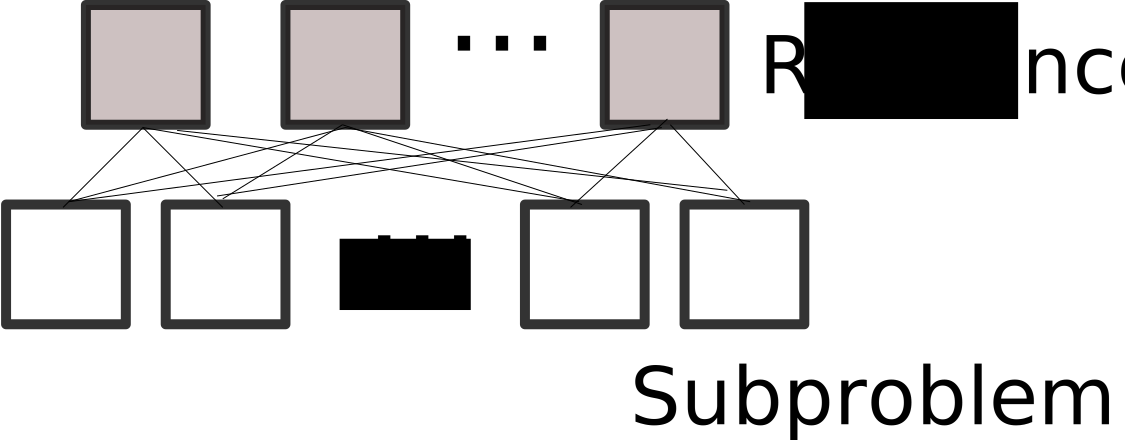
\includegraphics[width=0.7\linewidth]{fig/dependency}
\caption{The dependency of the trees in MORRF$^{*}$.}
\label{fig:dependency}
\end{figure}

Lemma \ref{lem:moo-d:rrt} tells us that the multi-objective path planning could be decomposed into a set of subproblems.
In MORRF$^{*}$, the responsibility of a subproblem tree is to find the optimal solution of its subproblem.
The next question needs to be answered is that whether the subproblem tree could find the optimal solution of its subproblem.

We notice that the \textsc{Extend} process in RRT$^{*}$ is not goal-oriented.
Let $ z^{*}(x) $ be the minimum cost from the start to the position of vertex $ x $.
We can generalize the conclusion of Theorem 22 in \cite{Karaman.Frazzoli:RSS10} to all the vertices in the RRT$^{*}$.
\begin{lem}
\label{lem:tree_vex:conv}
When Assumption \ref{asmp:additivity}, \ref{asmp:continuity} and \ref{asmp:spacing} hold,
the cost of the minimum cost path from the root to any vertex in RRT$^{*}$ converges to the optimal cost almost surely, i.e.,
$
P( \{ \lim_{ i \rightarrow \infty } c(x, i)  = z^{*}(x) \} ) = 1, x \in V $.
\begin{proof}
%The construction of RRT* is not goal-oriented.
%The ``rewire'' process potentially will update all the vertices and converge the value to the optimal one.
%Similar with that of a goal vertex, the paths from the root to all other vertices will converge to corresponding optimal ones as well.
The asymptotic optimality of RRT$^{*}$ does not rely on how the sampling process is like (Theorem 22, \cite{Karaman.Frazzoli:RSS10}), though the convergence rate might be different.
Simply changing the goal to the position of any vertex still hold the asymptotic optimality.
Thus, we could generalize the asymptotic optimality from the goal to all the vertices.
\end{proof}
\end{lem}

The solve of a subproblem depends on a correct estimation of the reference vector $ \vec{z}^{*} $.
Thus, we need to have the solutions of all the reference trees converging to the optimal firstly.
The construction of a reference tree does not depend on any other tree.
Thus, the construction process is equivalent to the construction of a RRT*.
The asymptotic optimality of RRT* in Lemma \ref{lem:tree_vex:conv} is inherited here.
Thus the cost of the solution converges to the optimal of single objective.
\begin{lem}
\label{lem:ref_tree:conv}
When Assumption \ref{asmp:additivity}, \ref{asmp:continuity} and \ref{asmp:spacing} hold,
the cost of the minimum cost path from the root to any vertex in $ k $-th reference tree converges to $ z^{*}_{k} $ almost surely, i.e., 
$ P( \{ \lim_{ i \rightarrow \infty }  c_{k} (x, i ) = z^{*}_{k} (x) \} ) = 1  $.
\end{lem}

Then we need to show that after all the reference trees converge to the structure that provides optimal cost, 
the subproblem tree can also converge to the structure that provides optimal fitness $ g^{*}_{m} ( x \mid \lambda_{m} , z^{*} ) $.
\begin{lem}
\label{lem:sub_tree:conv}
When Assumption \ref{asmp:additivity}, \ref{asmp:continuity} and \ref{asmp:spacing} hold,
with $ \vec{z}^{*} (x) $ for any $ x $ given,
the cost of the solution of $ m $-th subproblem tree converges to the optimal cost of the $ m $-th subproblem, i.e.,
$
P( \{ \lim_{ i \rightarrow \infty } c_{ \lambda_{m} }( i ) \} ) = z^{*}_{ \lambda_{m} }
$
\begin{proof}
When the reference vector $ \vec{z}^{*}(x) $ converges, the cost of the minimum cost path from the root to the vertex of position $ x $ in $ m $-th subproblem tree will gradually converge to the optimal by Lemma \ref{lem:tree_vex:conv}.
It means that the minimum fitness path from the root to any vertex in a subproblem tree will converge to an optimal minimum fitness path, in which the vertices in goal region are included.
It equals to that the cost of the solution of $ m $-th subproblem tree converges to the optimal cost of the $ m $-th subproblem.
%The construction of a subproblem tree depends on the convergence of all the reference trees.
%When all the reference trees have converged, the correct reference values $ c^{*} (x) $ of all the vertices could be obtained.
%The convergence process will be similar with that of a single RRT*.
%By Lemma \ref{lem:ref_tree:conv} and Lemma \ref{lem:sub_tree:conv}, we know that the utopia reference value $ c^{*} (x) $ could be correctly estimated after all the reference trees have reached optimality.
\end{proof}
\end{lem}

Now, we can prove that the solutions from MORRF$^{*}$ almost surely converges to a subset of the Pareto optimal set.

\begin{thm}
\label{thm:morrt:conv}
When Assumption \ref{asmp:additivity}, \ref{asmp:continuity} and \ref{asmp:spacing} hold,
the solutions from MORRF$^{*} $ converges to a subset of the Pareto optimal set almost surely, i.e.
$
P( \lim_{ i \rightarrow \infty }  \Sigma^{\mbox{MORRF}^{*}}_{i}  \subset \Sigma^{*} ) = 1.
$
\begin{proof}
As the solutions of MORRF$^{*}$ can be modeled in points in a high-dimension space by Lemma \ref{lem:moo-d:rrt}, the Tchebycheff method could be imported to decompose the multi-objective optimization problem into a set of subproblems.
By the fitness definition of the subproblem trees, if the subproblem tree could find a solution that minimize the fitness, the solution is in the Pareto optimal set of the multi-objective optimization problem.

Lemma \ref{lem:ref_tree:conv} guarantees that the reference vector $ \vec{z}^{*}(x) $ at any location $ x $ converges to the correct estimation after running enough iteration.
Thus, by Lemma \ref{lem:sub_tree:conv}, we have that the solution cost of the $ m $-th subproblem tree converges to $ z^{*}_{ \lambda_{m} } $.
It means that the solution converges to an optimal solution to $ m $-th subproblem as the iteration goes.
Therefore, the set of the solutions from all the subproblem trees converge to a subset of the Pareto optimal set, as the iteration goes~\cite{4358754}~\cite{miettinen1999nonlinear}.
\end{proof}
\end{thm}

\section{Simulation}
\label{sec:simulation}

\begin{comment}
2D (weighted sum + Tchebycheff method)
2D (With obstacles)
3D
compare NSGA-II
\end{comment}

Simulations have been taken to verify the performance of MORRF$^{*}$.
In order to compare the performance, we also implemented NSGA-II for multi-objective path planning, which is introduced in \cite{Ahmed2013}.
To make it comparable, the path planning using NSGA-II works in a continuous space and the solution format has been modified to a sequence of waypoints.
Thus the solution from the NSGA-II can have same format with those from MORRF$^{*}$.
The cost calculation is identical with that in  MORRF$^{*}$, whcih \textsc{Line}($ x_{1}, x_{2} $) is called to calculate the cost between two way points $ x_{1} $ and $ x_{2} $.

We have implemented two types of  MORRF$^{*}$, using different decomposition approaches, the weighted sum approach and the Tchebycheff approach.
The Tchebycheff approach depends on the knowledge of the reference vector, but the weighted sum approach does not.
However, the weighted sum approach works well only when all the objectives are convex~\cite{4358754}.
Also the Tchebycheff approach should bring better diversity in the solutions~\cite{4358754}.

All the methods run $ 5000 $ iterations and generate $ 30 $ solutions.
We tested firstly on path planning of two objectives.
One objective is  Euclidean distance minimization, the other objective is a given fitness minimization, as shown in Figure \ref{fig:sim:norm:distance} and \ref{fig:sim:norm:fitness1}.
The convergence of NSGA-II based path planning is very slow.
In Figure \ref{fig:sim:norm:pf:a}, a Pareto-front like fitness distribution is formed but the distance to the reference vector is much further away.
Weighted sum approach returns a set of solutions close to the Pareto optimal set in Figure \ref{fig:sim:norm:pf:b} and \ref{fig:sim:norm:sols:b}, but the Tchebycheff approach shows better diversity in Figure \ref{fig:sim:norm:pf:c} and \ref{fig:sim:norm:sols:c}.

\begin{figure}
	\centering
	\begin{subfigure}[b]{0.45\linewidth}
		\centering
		\includegraphics[width=\textwidth]{fig/sim2-2obj/MORRTstar00-0.png}
		\caption{Minimize distance}
		\label{fig:sim:norm:distance}
	\end{subfigure}
	\begin{subfigure}[b]{0.45\linewidth}
		\centering
		\includegraphics[width=\textwidth]{fig/sim2-2obj/MORRTstar00-1.png}
		\caption{Minimize fitness 1}
		\label{fig:sim:norm:fitness1}
	\end{subfigure}  \\
	\begin{subfigure}[b]{0.45\linewidth}
		\centering
		\includegraphics[width=\textwidth]{fig/sim3-2obj/PF03-MOPATH.png}
		\caption{Pareto front using NSGA-II}
		\label{fig:sim:norm:pf:a}
	\end{subfigure}
	\begin{subfigure}[b]{0.45\linewidth}
		\centering
		\includegraphics[width=\textwidth]{fig/sim3-2obj/MOPath01-ALL.png}
		\caption{Pareto optimal paths using NSGA-II}
		\label{fig:sim:norm:sols:a}
	\end{subfigure}  \\
	\begin{subfigure}[b]{0.45\linewidth}
		\centering
		\includegraphics[width=\textwidth]{fig/sim1-2obj/PF01-MORRT.png}
		\caption{Pareto front using weighted sum approach}
		\label{fig:sim:norm:pf:b}
	\end{subfigure}
	\begin{subfigure}[b]{0.45\linewidth}
		\centering
		\includegraphics[width=\textwidth]{fig/sim1-2obj/MORRTstar00-ALL.png}
		\caption{Pareto optimal paths using weighted sum approach}
		\label{fig:sim:norm:sols:b}
	\end{subfigure}  \\
	\begin{subfigure}[b]{0.45\linewidth}
		\centering
		\includegraphics[width=\textwidth]{fig/sim2-2obj/PF02-MORRT2.png}
		\caption{Pareto front using Tchebycheff approach}
		\label{fig:sim:norm:pf:c}
	\end{subfigure} 
	\begin{subfigure}[b]{0.45\linewidth}
		\centering
		\includegraphics[width=\textwidth]{fig/sim2-2obj/MORRTstar00-ALL.png}
		\caption{Pareto optimal paths using Tchebycheff approach}
		\label{fig:sim:norm:sols:c}
	\end{subfigure}
	\caption{Path planning with two objectives.}
	\label{fig:sim:norm}
\end{figure}

We also imported obstacles to the environment to see how the performance of the MORRTF$^{*}$ becomes.
The results are shown in Figure \ref{fig:sim:obs}.

\begin{figure}
	\centering
	\begin{subfigure}[b]{0.45\linewidth}
		\centering
		\includegraphics[width=\textwidth]{fig/sim4-obstacle/MORRTstar01-1-0.png}
		\caption{Minimize distance}
		\label{fig:sim:obs:distance}
	\end{subfigure}
	\begin{subfigure}[b]{0.45\linewidth}
		\centering
		\includegraphics[width=\textwidth]{fig/sim4-obstacle/MORRTstar01-1-1.png}
		\caption{Minimize fitness 1}
		\label{fig:sim:obs:fitness1}
	\end{subfigure}  \\
	\begin{subfigure}[b]{0.45\linewidth}
		\centering
		\includegraphics[width=\textwidth]{fig/sim4-obstacle/PF04-MORRT.png}
		\caption{Pareto front using weighted sum approach}
		\label{fig:sim:obs:pf:a}
	\end{subfigure}
	\begin{subfigure}[b]{0.45\linewidth}
		\centering
		\includegraphics[width=\textwidth]{fig/sim4-obstacle/MORRTstar01-1-ALL.png}
		\caption{Pareto optimal paths using weighted sum approach}
		\label{fig:sim:obs:sols:a}
	\end{subfigure}  \\
	\begin{subfigure}[b]{0.45\linewidth}
		\centering
		\includegraphics[width=\textwidth]{fig/sim5-obstacle/PF05-MORRT2.png}
		\caption{Pareto front using Tchebycheff approach}
		\label{fig:sim:obs:pf:b}
	\end{subfigure} 
	\begin{subfigure}[b]{0.45\linewidth}
		\centering
		\includegraphics[width=\textwidth]{fig/sim5-obstacle/MORRTstar01-1-ALL.png}
		\caption{Pareto optimal paths using Tchebycheff approach}
		\label{fig:sim:obs:sols:b}
	\end{subfigure}
	\caption{Path planning with two objectives and the obstacles.}
	\label{fig:sim:obs}
\end{figure}

We also tested the case that the two objectives exist mutual contradiction.
The two fitness distributions are given in Figure \ref{fig:sim:nonconvex:fitness1} and \ref{fig:sim:nonconvex:fitness2}.
The results are illustrated in Figure \ref{fig:sim:nonconvex}.
It is obvious that the result of Tchebycheff approach shows better diversity than that of the weighted sum approach in Figure \ref{fig:sim:nonconvex}.

\begin{figure}
	\centering
	\begin{subfigure}[b]{0.45\linewidth}
		\centering
		\includegraphics[width=\textwidth]{fig/sim8-nconvex/MORRTstar03-0.png}
		\caption{Minimize fitness 1}
		\label{fig:sim:nonconvex:fitness1}
	\end{subfigure}
	\begin{subfigure}[b]{0.45\linewidth}
		\centering
		\includegraphics[width=\textwidth]{fig/sim8-nconvex/MORRTstar03-1.png}
		\caption{Minimize fitness 2}
		\label{fig:sim:nonconvex:fitness2}
	\end{subfigure}  \\
	\begin{subfigure}[b]{0.45\linewidth}
		\centering
		\includegraphics[width=\textwidth]{fig/sim8-nconvex/PF03-MORRT.png}
		\caption{Pareto front using weighted sum approach}
		\label{fig:sim:nonconvex:pf:a}
	\end{subfigure}
	\begin{subfigure}[b]{0.45\linewidth}
		\centering
		\includegraphics[width=\textwidth]{fig/sim8-nconvex/MORRTstar03-ALL.png}
		\caption{Pareto optimal paths using weighted sum approach}
		\label{fig:sim:nonconvex:sols:a}
	\end{subfigure}  \\
	\begin{subfigure}[b]{0.45\linewidth}
		\centering
		\includegraphics[width=\textwidth]{fig/sim9-nconvex/PF03-MORRT2.png}
		\caption{Pareto front using Tchebycheff approach}
		\label{fig:sim:nonconvex:pf:b}
	\end{subfigure} 
	\begin{subfigure}[b]{0.45\linewidth}
		\centering
		\includegraphics[width=\textwidth]{fig/sim9-nconvex/MORRTstar03-ALL.png}
		\caption{Pareto optimal paths using Tchebycheff approach}
		\label{fig:sim:nonconvex:sols:b}
	\end{subfigure}
	\caption{Path planning with two conflict objectives.}
	\label{fig:sim:nonconvex}
\end{figure}

In order to verify how the MORRF$^{*}$ performs with more objectives, we tested a case with three objectives.
The Euclidean distance is the first objective, the other two objectives are shown in Figure \ref{fig:sim:many:fitness1} and \ref{fig:sim:many:fitness2}.
The results are given in Figure \ref{fig:sim:many}.
We can see that the Pareto front has formed towards the reference vector (Green point) in Figure \ref{fig:sim:many:pf:a} and \ref{fig:sim:many:pf:b}.

\begin{figure}
	\centering
	\begin{subfigure}[b]{0.31\linewidth}
		\centering
		\includegraphics[width=\textwidth]{fig/sim6-3obj/MORRTstar02-0.png}
		\caption{Minimize distance}
		\label{fig:sim:many:distance}
	\end{subfigure}
	\begin{subfigure}[b]{0.31\linewidth}
		\centering
		\includegraphics[width=\textwidth]{fig/sim6-3obj/MORRTstar02-1.png}
		\caption{Minimize fitness 1}
		\label{fig:sim:many:fitness1}
	\end{subfigure}
	\begin{subfigure}[b]{0.31\linewidth}
		\centering
		\includegraphics[width=\textwidth]{fig/sim6-3obj/MORRTstar02-2.png}
		\caption{Minimize fitness 2}
		\label{fig:sim:many:fitness2}
	\end{subfigure}  \\
	\begin{subfigure}[b]{0.45\linewidth}
		\centering
		\includegraphics[width=\textwidth]{fig/sim6-3obj/PF06-MORRT.png}
		\caption{Pareto front using weighted sum approach}
		\label{fig:sim:many:pf:a}
	\end{subfigure}
	\begin{subfigure}[b]{0.45\linewidth}
		\centering
		\includegraphics[width=\textwidth]{fig/sim6-3obj/MORRTstar02-ALL.png}
		\caption{Pareto optimal paths using weighted sum approach}
		\label{fig:sim:many:sols:a}
	\end{subfigure}  \\
	\begin{subfigure}[b]{0.45\linewidth}
		\centering
		\includegraphics[width=\textwidth]{fig/sim7-3obj/PF07-MORRT2.png}
		\caption{Pareto front using Tchebycheff approach}
		\label{fig:sim:many:pf:b}
	\end{subfigure} 
	\begin{subfigure}[b]{0.45\linewidth}
		\centering
		\includegraphics[width=\textwidth]{fig/sim7-3obj/MORRTstar02-ALL.png}
		\caption{Pareto optimal paths using Tchebycheff approach}
		\label{fig:sim:many:sols:b}
	\end{subfigure}
	\caption{Path planning with three objectives.}
	\label{fig:sim:many}
\end{figure}

\section{Conclusion} 
\label{sec:conclusion}

This paper presented a MORRF$^{*}$ for the multi-objective path planning problems on continuous spaces.
The multi-objective path planning problem is decomposed into a few subproblems.
Each subproblem is assigned to a subproblem tree of a forest.
The subproblem trees parallel explore the working space by same new sampling positions.
Analyses have shown that the solutions of all the subproblem trees is a subset of the Pareto optimal solutions.
Experiments have been taken to verify the effectiveness and evaluate the performance of the MORRF$^{*}$.

In the experiment, only weighted sum approach and the Tchebycheff approach have been tested. 
It is obvious that the solutions from Tchebycheff approach shows better diversity than those from weighted sum approach.
It is expected that the solutions from Boundary intersection approach would have even better diversity.

There is also a lot of space to improve the efficiency of MORRT$^{*} $.
Importing more prior should help to reduce some redundant samplings, which accelerates the convergence.
Currently the sampling is still uniformly random.
We can do the sampling based on the information collected from the environment, more efforts can then be put in the more interesting regions.

If we take a goal position as the root to extend using MORRT$^{*}$,
we should be able to find a similar set of Pareto optimal paths.
In this case, if the movement deviates from the original paths, it is very efficient to get a new set of Pareto optimal paths from the new position to the goal position.
Because the convergence of MORRT$^{*}$ means the optimal paths from all the vertices to the root.


\section*{Acknowledgments}

%% Use plainnat to work nicely with natbib. 

\bibliographystyle{plainnat}
\bibliography{reference}

\end{document}